% !TEX root = ../agglo_clust_review.tex

\begin{figure}[t]
\centering
% 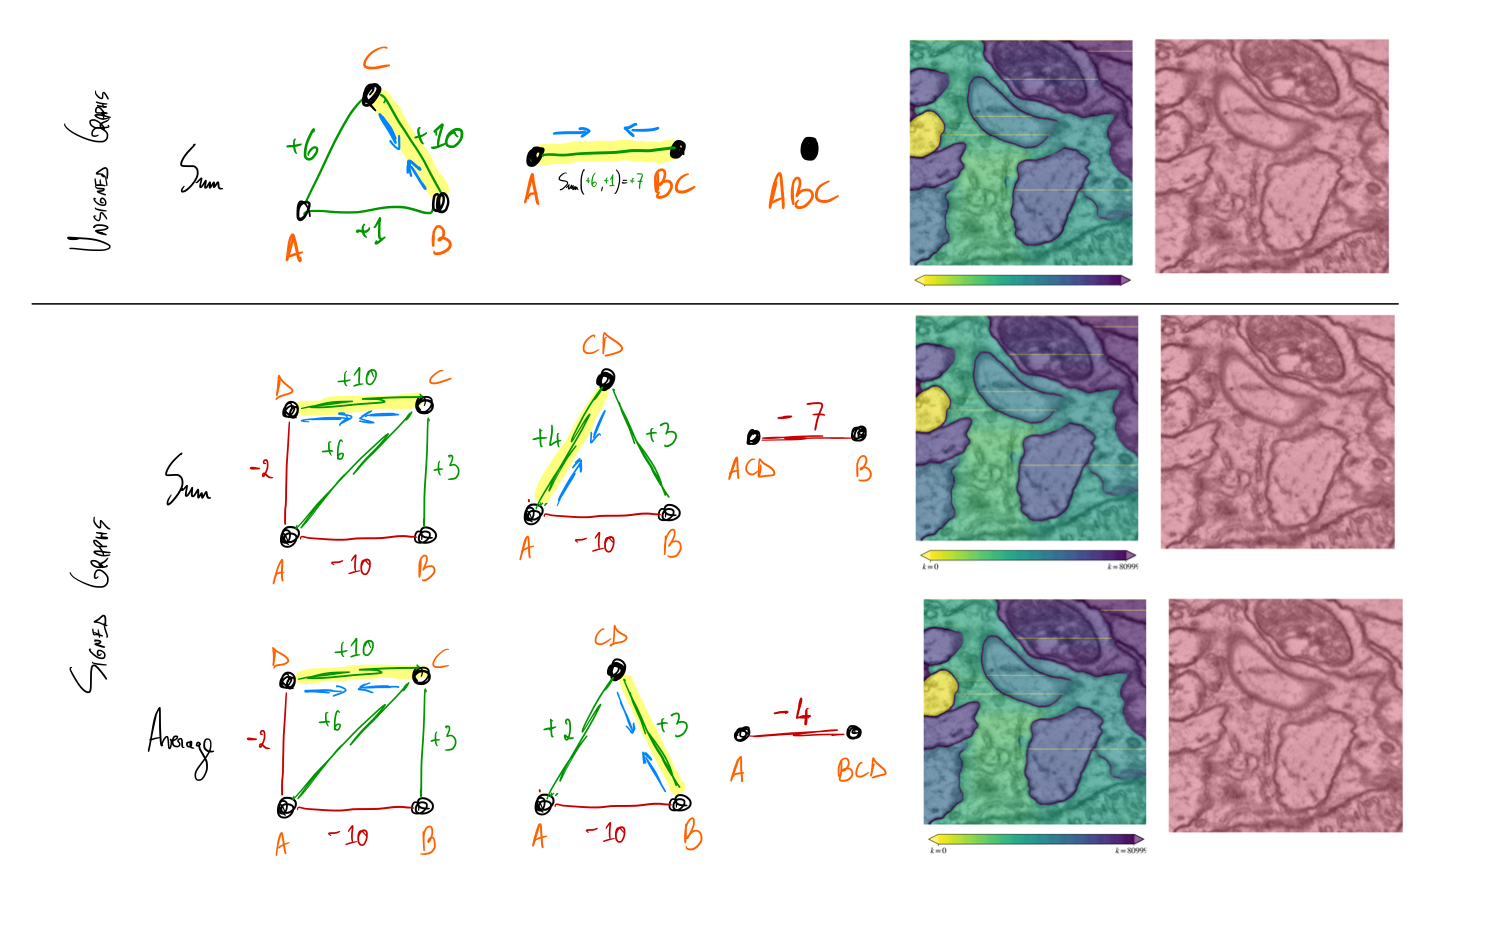
\includegraphics[width=0.5\textwidth,trim=0.4in 1.2in 0.in 0.05in,clip]{./figs/intro_image.jpg} % left bottom right top
\includegraphics[width=\textwidth]{./figs/comparison.pdf} % left bottom right top
\caption{
\UPDATE{Comparison of results from different update rules on signed graph with and without cannot-link constraints 
}
 % main ideas and contributions
\label{fig:cremi_comparison}}
\end{figure}

\section{Experiments on neuron segmentation}\label{sec:neuro_segm_exp}

We first evaluate and compare the agglomerative clustering algorithms described in the generalized framework on the task of neuron segmentation in electron microscopy (EM) image volumes. This application is of key interest in connectomics, a field of neuro-science with the goal of reconstructing neural wiring diagrams spanning complete central nervous systems. While a lot of progress is being made, only proof-reading or manual tracing yields sufficient accuracy for correct circuit reconstruction \cite{schlegel2017learning}.
\TODO{subsections description}

\subsection{Experimental setup: pixel grid-graph with long-range connections} \label{sec:grid_graph}
EM segmentation is commonly performed by first predicting which pixels belong to a cell membrane using a CNN. As described in Sec. \ref{sec:related_work}, different postprocessing methods are then used to obtain a segmentation. The CNN can either be trained to predict boundary pixels \cite{beier2017multicut,ciresan2012deep} or undirected affinities \cite{wolf2018mutex,lee2017superhuman,funke2018large}, which represent how likely it is for a pixel and one of its neighbors to belong to the same neuron segment. The affinities do not have to be limited to direct neighboring pixels, in fact, \cite{lee2017superhuman} have shown that using long-range affinities is beneficial for the training of the CNN. Similarly to \cite{wolf2018mutex}, we then train a CNN to predict short- and long-range affinities and use them as input weights for \algname{}. The output layer of the CNN will then have $m_{\mathrm{direct}}+m_{\mathrm{long}}$ channels, where $m_{\mathrm{direct}}=6$ represents the direct neighbors in 3D and $m_{\mathrm{long}}$ is the number of long-range ones. In the Supplementary material (Sec. \ref{sec:training_details}) we provide more details on the chosen neighborhood structure, data augmentation and the training with L1 loss of the used 3D U-Net architecture \cite{ronneberger2015u,cciccek20163d}.

The output of the CNN can be represented as a weighted 3D grid graph, such that each node represents a pixel/voxel of the volume image. Each node is connected to its neighbors by $m_{\mathrm{direct}}$ edges ($E_{\mathrm{direct}}$) and $m_{\mathrm{long}}$ long-range ones ($E_{\mathrm{long}}$).
In our experiments we evaluate how beneficial long-range connections are for the final segmentation and we add them to the graph with a given probability $p_{\mathrm{long}}$ (if $p_{\mathrm{long}}=0$, then $E_{\mathrm{long}}=\emptyset$).
We note that the post-processing presented in \cite{lee2017superhuman} did not use any predicted long-range connection, whereas \cite{wolf2018mutex} introduced them with strides of 2 in the XY-plane.

The trained CNN outputs pseudo-probabilities $p:E \rightarrow [0,1]$ that have to be mapped to positive and negative edge weights\footnote{Note that in general attractive and repulsive interactions $w^+$ and $w^-$ can be independently estimated with different classifiers.}. The most common approaches use \emph{additive} \cite{ailon2008aggregating} or \emph{logarithmic} \cite{finkel2008enforcing,andres2012globally} mappings:
\begin{equation}
\cost_{e,\mathrm{Add}} = p_e - \beta, \qquad \quad \cost_{e,\mathrm{Log}} = \log \left( \frac{p_e}{1-p_e} \right) + \log \left( \frac{\beta}{1-\beta} \right),
\end{equation}
where $\beta \in [0,1]$ is a \emph{bias} parameter that allow a tuning between over- and under-segmentation. We evaluated both of them empirically with each of the tested linkage and found that the additive mapping is the best option in all cases apart from the \emph{Sum} linkage. 
